\documentclass{article}


% if you need to pass options to natbib, use, e.g.:
%     \PassOptionsToPackage{numbers, compress}{natbib}
% before loading neurips_2023


% ready for submission
\usepackage[]{neurips_2023}


% to compile a preprint version, e.g., for submission to arXiv, add add the
% [preprint] option:
%     \usepackage[preprint]{neurips_2023}


% to compile a camera-ready version, add the [final] option, e.g.:
%     \usepackage[final]{neurips_2023}


% to avoid loading the natbib package, add option nonatbib:
%    \usepackage[nonatbib]{neurips_2023}


\usepackage[utf8]{inputenc} % allow utf-8 input
\usepackage[T1]{fontenc}    % use 8-bit T1 fonts
\usepackage{hyperref}       % hyperlinks
\usepackage{url}            % simple URL typesetting
\usepackage{booktabs}       % professional-quality tables
\usepackage{amsfonts}       % blackboard math symbols
\usepackage{nicefrac}       % compact symbols for 1/2, etc.
\usepackage{microtype}      % microtypography
\usepackage{xcolor}         % colors
\usepackage{multirow}
\usepackage{graphicx}       % include images
\usepackage{caption}
\usepackage{algorithm}
\usepackage{algorithmic}
\usepackage{amsmath}
\usepackage{amssymb}
\usepackage{amsthm}

% Images folder


\title{Unsupervised Domain Adaptation}


% The \author macro works with any number of authors. There are two commands
% used to separate the names and addresses of multiple authors: \And and \AND.
%
% Using \And between authors leaves it to LaTeX to determine where to break the
% lines. Using \AND forces a line break at that point. So, if LaTeX puts 3 of 4
% authors names on the first line, and the last on the second line, try using
% \AND instead of \And before the third author name.


\author{ Krishna Agarwal\\%\thanks{Use footnote for providing further information
    %about author (webpage, alternative address)---\emph{not} for acknowledging
    %funding agencies.} \\
  Indian Institute of Science, Bangalore\\
  \texttt{krishnaagarw@iisc.ac.in} \\
  % examples of more authors
   \And
  {Pratham Gupta} \\
  Indian Institute of Science, Bangalore\\
  \texttt{prathamgupta@iisc.ac.in} \\
   \And
   {Gavish Bansal} \\
   Indian Institute of Science, Bangalore\\
   \texttt{gavishbansal@iisc.ac.in} \\
   \And
   {Kintan Saha} \\
   Indian Institute of Science, Bangalore\\
   \texttt{kintansaha@iisc.ac.in} \\
  % \And
  % Coauthor \\
  % Affiliation \\
  % Address \\
  % \texttt{email} \\
}


\begin{document}
\graphicspath{{./images/}}

\maketitle


\begin{abstract}
  
\end{abstract}


\section{Introduction}
Unsupervised domain adaptation (UDA) is a type of domain adaptation in machine learning where a model is trained on a source domain with labelled data, and then adapted to a target domain with unlabelled data.
In UDA, the source domain and target domain have different distributions, but
the goal is to leverage the labelled data in the source domain to improve performance on the target
domain. \\
This report is product of our exploration of state of the art UDA algorithms and their applications in various fields like computer vision, natural language processing, etc. 
We have reproduced the results of these key papers [] in this research area of machine learning.

\section{Methodology}

\subsection{Algorithms}
We have implemented the following algorithms for our experiments:
\begin{itemize}
  \item \textbf{DANN (Domain-Adversarial Neural Network)}[]: Trains the model in an adversarial manner to learn the domain invariant features using a gradient reversal layer and a DNN.
  \item \textbf{CORAL (Correlation Alignment), DeepCORAL}[][]: CORAL aligns the second-order statistics (covariances) of source and target features. Accordingly, DeepCORAL is an extension of CORAL that integrates correlation alignment into deep neural networks.
  \item \textbf{MMD (Maximum Mean Discrepancy)}[]: A metric that quantifies non-alignment between the source and target distributions. It is used as a loss function and in validating models. 
  \item \textbf{DSN (Domain Separation Network)}[]: Separates domain-specific and domain-invariant features for better adaptation. A state of the art method for domain invariant feature learning.
  \item \textbf{ATT (Adversarial Training with Triplet loss)}[]:An ensemble method that utilize two classifier trained on source domain to pseudo-label target domain to learn a classifier for it.
\end{itemize}

\subsection{Datasets}
We have used the following datasets\ref{tab:datasets} for our experiments:
\begin{table}[h]
  \centering
  \caption{Benchmark datasets used in our experiments.}
  \label{tab:datasets}
  \begin{tabular}{ll}
      \toprule
      \textbf{Dataset Category} & \textbf{Datasets} \\
      \midrule
      Computer Vision (Numbers)     & MNIST, MNIST-M, SVHN \\
      Computer Vision (Categorical) & Office: Amazon, DSLR, Webcam \\
      Sentiment Analysis (Classification)  & Amazon Review Sentiment \\
      \bottomrule
  \end{tabular}
\end{table}


\section{Experiments}
\subsection{CORAL and DeepCORAL}
\subsubsection{CORAL}

\subsubsection{DeepCORAL}
We have implemented the DeepCORAL algorithm and observed its performance in domain adaptation using the Office dataset, taking every combination of domains as source and target. The results are shown in Table \ref{tab:deepcoral}. Note that we also compare our results with the results mentioned in the survey paper[]. It is observable that the result for \textbf{W}$\rightarrow$ \textbf{A} is in disagreement with the result in the survey paper by approximately 4\%. The plausible reasons for this discrepancy have been mentioned in the Appendix.
 
\begin{table*}
  \caption{Classification accuracy (source $\rightarrow$ target) of DeepCORAL on the Office computer vision dataset. A: Amazon, D: DSLR, W: Webcam.}
  \label{comparePerformance2}
  \begin{scriptsize}
  \begin{center}
  {\renewcommand{\arraystretch}{1.4}
  \begin{tabular}{@{}l cccccc@{}}
  \toprule
  \multicolumn{1}{c}{\multirow{2}{*}{\textbf{Result Source}}} & \multicolumn{6}{c}{\textbf{Office (Amazon, DSLR, Webcam)}} \\
  \cmidrule{2-7}
   & \textbf{A $\rightarrow$ W} & \textbf{D $\rightarrow$ W} & \textbf{W $\rightarrow$ D} & \textbf{A $\rightarrow$ D} & \textbf{D $\rightarrow$ A} & \textbf{W $\rightarrow$ A} \\
  \midrule
  \textbf{Our Code} & 62.05 & 95.32 & 99.56 & 64.44 & 52.77 & 56.49\\
  \hline
  \textbf{Survey Paper} & 66.4$\pm$0.4 & 95.7$\pm$0.3 & 99.2$\pm$0.1 & 66.8$\pm$0.6 & 52.8$\pm$0.2 & 51.5$\pm$0.3\\
  \bottomrule
  \end{tabular}
  }
  \end{center}
  \end{scriptsize}
  \label{tab:deepcoral}
\end{table*}

\subsection{Maximum Mean Discrepancy}
Similar to DeepCORAL, we also experimented by taking MMD as our divergence metric. We have used synthetic dataset to test the performance of MMD and it showed good good ability to adapt as shown in figure \ref{fig:mmd}. We empirically verified MMD's ability to distinguish between different distributions \ref{fig:mmd_power}. By testing on synthetically generated data\ref{fig:mmd_example}. 

\begin{figure}
  \centering
  \begin{minipage}{0.3\textwidth}
    \centering
    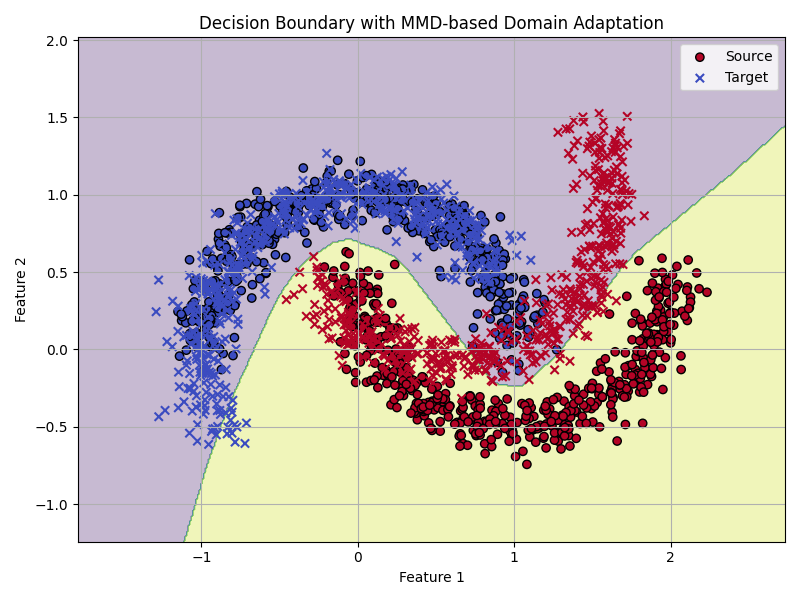
\includegraphics[width=\textwidth]{MMD/adaptation.png}
    \caption{Plot of desicion boundary of DNN trained with MMD loss. The decision boundary is shown for the source domain (dots) and target domain (cross).}
    \label{fig:mmd}
  \end{minipage}
  \hfill
  \begin{minipage}{0.35\textwidth}
    \centering
    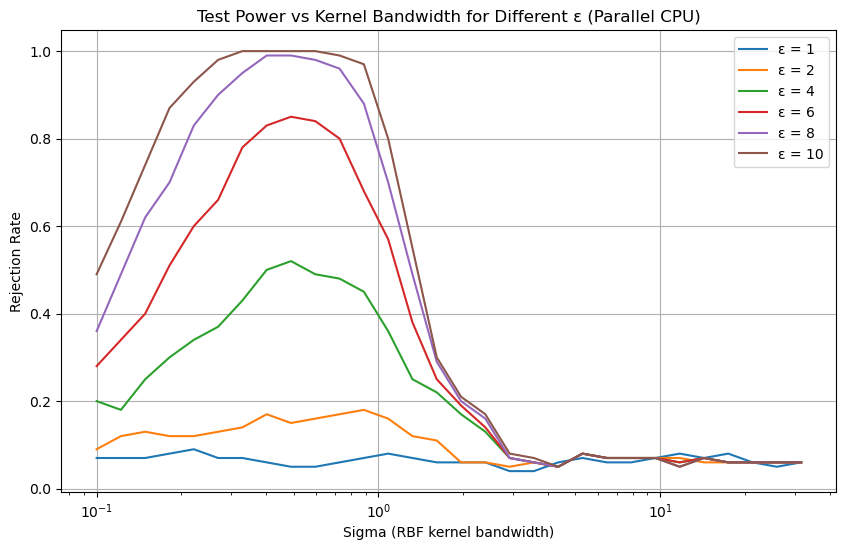
\includegraphics[width=\textwidth]{MMD/Test_powe_vs_eps.png}
    \caption{MMD: Test power vs epsilon shows how well MMD can distinguish between distributions vs how much they differ.}
    \label{fig:mmd_power}
  \end{minipage}
  \hfill
  \begin{minipage}{0.25\textwidth}
    \centering
    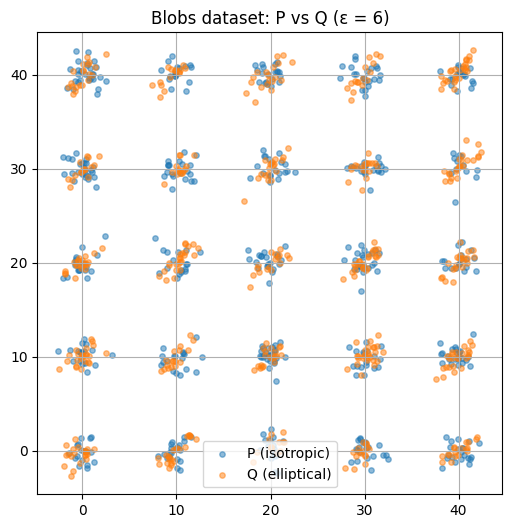
\includegraphics[width=\textwidth]{MMD/Example.png}
    \caption{Example of synthetic dataset, where P is Isotropic Gaussian while Q is elliptical.}
    \label{fig:mmd_example}
  \end{minipage}
  

\end{figure}


\subsection{Domain Separation Network}
We have implemented the DSN algorithm and observed its performance in domain adaptation using the MNIST and MNIST-M datasets. Our Resulting accuracy is shown in Table \ref{tab:dsn}. The results are comparable to the results mentioned in the paper. Further more we can also observe the reconstructed images from the DSN model. The reconstructed images are shown in figure \ref{fig:dsn_reconstruction}.




\begin{figure}
  \centering
  % First minipage: the table
  \begin{minipage}[t]{0.45\textwidth}
    \centering
    \begin{minipage}[t]{0.95\textwidth}
      \centering
      \captionof{table}{Results of DSN on MNIST and MNIST-M Domain Adaptation.}
      \label{tab:dsn}
      \begin{tabular}{lc}
        \toprule
        \textbf{Method} & \textbf{Accuracy} \\
        \midrule
        DSN (Ours) & 81.6\% \\
        DSN (Paper) & 83.2\% \\
        \bottomrule
      \end{tabular}
    \end{minipage}
    \vspace{2mm}
    \begin{minipage}[t]{0.95\textwidth}
      \vspace{4mm}
      \centering
      \begin{minipage}[t]{0.95\textwidth}
        \centering
        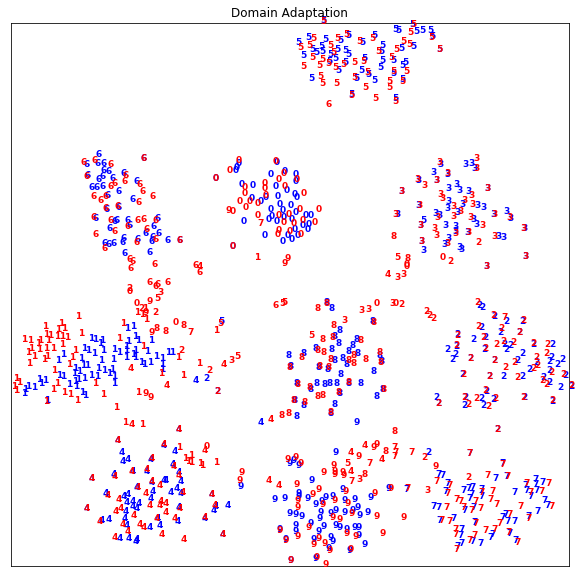
\includegraphics[width=0.75
        \linewidth]{DSN/DNS_MNIST_MNISTM.png}
        \caption{@krishna Put the caption here}
      \end{minipage}
    \end{minipage}
  \end{minipage}%
  \hfill
  % Second minipage: the 2x2 image grid
  \begin{minipage}[t]{0.5\textwidth}
    \caption{Reconstructed images from DSN.}
    \label{fig:dsn_reconstruction}
    \centering
    \begin{minipage}[t]{0.48\textwidth}
      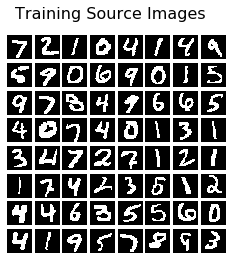
\includegraphics[width=\linewidth]{DSN/source.png}
    \end{minipage}
    \hfill
    \begin{minipage}[t]{0.48\textwidth}
      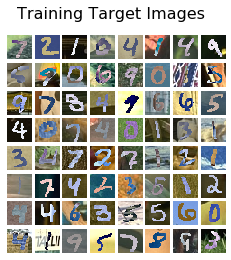
\includegraphics[width=\linewidth]{DSN/target.png}
    \end{minipage}
    \vspace{2mm}
    \begin{minipage}[t]{0.48\textwidth}
      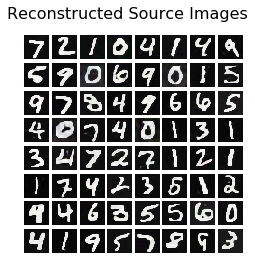
\includegraphics[width=\linewidth]{DSN/reconstructed_source.png}
    \end{minipage}
    \hfill
    \begin{minipage}[t]{0.48\textwidth}
      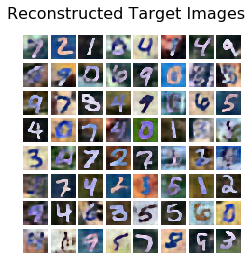
\includegraphics[width=\linewidth]{DSN/reconstructed_target.png}
    \end{minipage}

  \end{minipage}
\end{figure}



\subsection{Asymmetric Tri-training for Unsupervised Domain Adaptation}
We have Implement Asymmetric Tri-Training Algorithm and Tested it on MNIST and SVHN datasets. Results are shown in Table \ref{tab:att_results}. The results are comparable to the results mentioned in the paper. We have also compared our implementation with the implementation of the paper. The results are shown in Table \ref{tab:att_results}. It is observable that our implementation closely matched for training without batch normalization but other experiments fell short from the implementation of the paper. The plausible reasons for this discrepancy is insufficient training time and hyperparameter tuning.
\begin{table}
  \centering
  \caption{Results of ATT on MNIST and SVHN Domain Adaptation.}
  \label{tab:att_results}
  \begin{tabular}{lccc}
      \toprule
      \textbf{Method} & \textbf{MNIST\(\to\)SVHN} & \textbf{SVHN \(\to\) MNIST} \\
      \midrule
      Our w/o Batch Normalization & 36.9\% & 76.8\% \\
      Ours w/o Multi-view Loss & 15.2\% & 76.5\% \\
      Ours  & 15.2\% & 71.4\% \\
      \midrule
      Papers w/o Batch Normalization & 39.8\% & 79.8\% \\
      Papers w/o Multi-view Loss & 49.7\% & 86.0\% \\
      Papers  & 52.8\% & 85.8\% \\
      \bottomrule
  \end{tabular}
\end{table}


% \begin{figure}[h]
%   \centering
%   \includegraphics[width=0.5\textwidth]{ATT_Architecture.png}
%   \caption{ATT Architecture: The feature extractor F takes input from both source and target domain. F1 and F2 are classifiers trained on source domain. Ft is trained on target domain using pseudo-labels from F1 and F2.}
%   \label{fig:att_architecture}
% \end{figure}



\section{Conclusion}

In this report, we explored and implemented various state-of-the-art algorithms for Unsupervised Domain Adaptation (UDA), including DANN, CORAL, DeepCORAL, MMD, DSN, and ATT. Through rigorous experimentation across diverse benchmark datasets such as MNIST, SVHN, Office, and Amazon Reviews, we analyzed the performance and adaptability of these methods in different domain shift scenarios.

Our empirical results not only corroborate the findings from existing literature but also provide insights into implementation-level nuances that affect adaptation performance. For instance, our DeepCORAL results matched closely with prior work except for certain domain pairs, highlighting the importance of implementation details and preprocessing steps. Similarly, MMD-based models demonstrated strong distribution alignment capabilities, while DSN provided an interpretable approach via domain-specific reconstructions. For ATT, we observed that our implementation required more fine-tuning and compute resources to match the performance of the original paper, indicating the complexity of ensemble methods in UDA.

Overall, our work provides a comparative perspective on multiple UDA techniques and offers a reproducible framework for future researchers to build upon.

\newpage
\section*{Appendix}

\subsection*{Maximum Mean Discrepancy}
\subsubsection*{Theory}
Maximum Mean Discrepancy (MMD) is a statistical test used to measure the distance between two probability distributions. It is particularly useful in domain adaptation tasks where the goal is to align the feature distributions of the source and target domains. MMD computes the distance between the means of the two distributions in a reproducing kernel Hilbert space (RKHS). The MMD can be expressed mathematically as:
\[
  \text{MMD}^2(P, Q) = \left\| \frac{1}{m} \sum_{i=1}^{m} \phi(x_i) - \frac{1}{n} \sum_{j=1}^{n} \phi(y_j) \right\|^2_{\mathcal{H}}
\]
where \(P\) and \(Q\) are the two distributions, \(\phi\) is a feature map that maps the data into a high-dimensional space, and \(\mathcal{H}\) is the RKHS. The MMD can be computed using a kernel function, such as the Gaussian kernel, which allows for efficient computation in high-dimensional spaces. 
Formula for MMD is given as:
\[
  \text{MMD}^2(P, Q) = \mathbb{E}_{x,x'}[k(x,x')] + \mathbb{E}_{y,y'}[k(y,y')] - 2\mathbb{E}_{x,y}[k(x,y)]
\]
where \(k\) is the kernel function, and \(x\) and \(y\) are samples from the distributions \(P\) and \(Q\), respectively. 

An empirical estimate of MMD can be computed using the following formula:
\[
  \widehat{\text{MMD}}^2(P, Q) = \frac{1}{m(m-1)} \sum_{i=1}^{m} \sum_{j \neq i}^{m} k(x_i, x_j) + \frac{1}{n(n-1)} \sum_{i=1}^{n} \sum_{j \neq i}^{n} k(y_i, y_j) - \frac{2}{mn} \sum_{i=1}^{m} \sum_{j=1}^{n} k(x_i, y_j)
\]
From this we can define the test statistic as:
\[
  T = \frac{\widehat{\text{MMD}}^2(X,Y)}{\sqrt{\hat{V_m}(X,Y)}}
\]
where \(\widehat{V_m}(X,Y)\) is the variance of the MMD estimate. The null hypothesis is that the two distributions are equal, and the alternative hypothesis is that they are different. The test statistic \(T\) follows a standard normal distribution under alternate hypothesis \(H_1: P \neq Q\).

\[
  \frac{\widehat{\text{MMD}^2}_U(X,Y) - \text{MMD}^2(P,Q)}{\sqrt(T_m(P,Q))} \xrightarrow{d} \mathcal{N}(0,1)
\]

\subsubsection*{Implementation}
\textbf{Experiments of MMD as a divergence metric:}\\
We Implemented unbiased estimator of MMD and then generated blob data with different distributions. P and Q are \(5 \times 5\) grid of gaussian blobs where covariance of blobs are given by: \\
\begin{minipage}{0.45\linewidth}
\[
  P_{cov} = \begin{bmatrix}
    1 & 0 \\
    0 & 1
  \end{bmatrix}\sigma^2
\]
\end{minipage}
\hfill
\begin{minipage}{0.45\linewidth}
\[
  Q_{cov}(\epsilon) = \begin{bmatrix}
    1 & \frac{\epsilon-1}{\epsilon+1} \\
    \frac{\epsilon-1}{\epsilon+1} & 1
  \end{bmatrix} \sigma^2
\]
\end{minipage}

For a visual demonstration, Figure \ref{fig:mmd_example} shows an example where P is an isotropic Gaussian distribution (blue dots) and Q is an elliptical Gaussian distribution (orange dots) with \(\epsilon = 6\). 

To test the power of test statistic, we generated we used permutation test to compute the p-value. The p-value is computed as the fraction of times the test statistic is greater than the null statistic generated by taking the 95th percentile of the permuted combined samples. If mmd is able to distinguish between the two distributions then the number of rejections should be higher which is shown in figure \ref{fig:mmd_power}.

\textbf{MMD in Domain Adaptation:}\\
We used MMD as a divergence metric to train feature extractor and classifier. We tested it on Synthetic Moons data where target domain was rotated by 30 degrees. The feature extractor is a DNN with 2 hidden layers and ReLU activations. The classifier is a fully connected layer with softmax activation. The loss function is the sum of the cross-entropy loss and the MMD loss:
\[
  \mathcal{L}(\theta_F, \theta_C) = \mathcal{L}_{CE}(C(F(x_s)), y_s) + \lambda \cdot \text{MMD}^2(F(x_s), F(x_t))
\]
where \(\mathcal{L}_{CE}\) is the cross-entropy loss, \(C\) is the classifier, \(F\) is the feature extractor, and \(\lambda\) is a hyperparameter that controls the trade-off between the two losses. The MMD loss encourages the feature distributions of the source and target domains to be similar, thereby improving the model's performance on the target domain.
We trained the model 1200 epochs and used \(\lambda = 0.5\) and optimizer was Adam with learning rate of 0.001. Image of the decision boundary is shown in figure \ref{fig:mmd}.


\subsection*{Asymmetric Tri-training for Unsupervised Domain Adaptation}
\subsubsection*{Theory}
The Asymmetric Tri-training algorithm is a domain adaptation method that leverages multiple classifiers to improve the performance of a model on a target domain. The key idea is to use two classifiers trained on the source domain to generate pseudo-labels for the target domain, and then use these pseudo-labels to train a third classifier. 

The algorithm works in three main steps:

\begin{enumerate}
  \item \textbf{Source Domain Training}: Two classifiers (F1 and F2) are trained on labeled source domain data.
  
  \item \textbf{Pseudo-labeling}: F1 and F2 are used to predict labels for unlabeled target domain data. Only instances where both classifiers agree with high confidence are selected for pseudo-labeling.
  
  \item \textbf{Target Classifier Training}: A third classifier (Ft) is trained on the pseudo-labeled target domain data, incorporating a multi-view loss to ensure consistency between predictions.
\end{enumerate}

Complete Architecture is shown in figure \ref{fig:att_architecture}.

\textbf{Loss Functions:}\\
 The loss function for Source domain training is the cross-entropy loss + multi-view loss:
\[
  \mathcal{L}(\theta_F, \theta_{F_1}, \theta_{F_2}) = \mathcal{L}_{CE}(F_1(x_s), {y}_s) + 
  \mathcal{L}_{CE}(F_2(x_s), {y}_s) + \lambda
  \|W_1^T W_2\|
\]
The loss function for Target domain training is the cross-entropy loss:
\[
  \mathcal{L}(\theta_F, \theta_{F_t}) = \mathcal{L}_{CE}(F_t(x_t), \hat{y}_t)
\]

\begin{figure}[h]
  \centering
  \includegraphics[width=0.8\textwidth]{ATT/ATT_Architecture.png}
  \caption{ATT Architecture: The feature extractor F processes inputs from both domains. F1 and F2 are source-trained classifiers that generate pseudo-labels for training Ft on the target domain.}
  \label{fig:att_architecture}
\end{figure}

\subsubsection*{Pseudocode}
\begin{algorithm}[H]
\caption{Asymmetric Tri-training}
\begin{algorithmic}[1]
\STATE \textbf{Input:} Source data $X_s = \{(x_i, t_i)\}_{i=1}^m$, Target data $X_t = \{(x_j)\}_{j=1}^n$
\STATE $X_t^l = \emptyset$ \COMMENT{Initialize labeled target set}
\FOR{$j = 1$ to $iter$}
  \STATE Train $F, F_1, F_2, F_t$ with mini-batch from training set $S$
\ENDFOR
\STATE $N_t = N_{init}$
\STATE $X_t^l = \text{Labeling}(F, F_1, F_2, X_t, N_t)$
\STATE $L = X_s \cup X_t^l$
\FOR{$K$ steps}
  \FOR{$j = 1$ to $iter$}
    \STATE Train $F, F_1, F_2$ with mini-batch from training set $L$
    \STATE Train $F, F_t$ with mini-batch from training set $X_t^l$
  \ENDFOR
  \STATE $X_t^l = \emptyset$, $N_t = K/20 * n$
  \STATE $X_t^l = \text{Labeling}(F, F_1, F_2, X_t, N_t)$
  \STATE $L = X_s \cup X_t^l$
\ENDFOR
\end{algorithmic}
\end{algorithm}

\subsection*{Implementation Details}
We implemented the Asymmetric Tri-training algorithm using PyTorch. The model architecture (fig\ref{fig:att_implementation}) consists of a feature extractor followed by three classifiers. The feature extractor is a convolutional neural network (CNN) for image data, while the classifiers are fully connected layers. We used momentum SDG with a learning rate of 0.01 and momentum 0.9 and a batch size of 128. Lamda was set to 0.01 for the multi-view loss. We trained for 20 iters and value of K as 50. This computation required 2-3 hours of training time on GPU hence we were not able to train it for the recommened 2000 iterations as mentioned in the paper. Which we believe is the reason for the discrepancy in results as compared to the paper.
\begin{figure}[h]
  \centering
  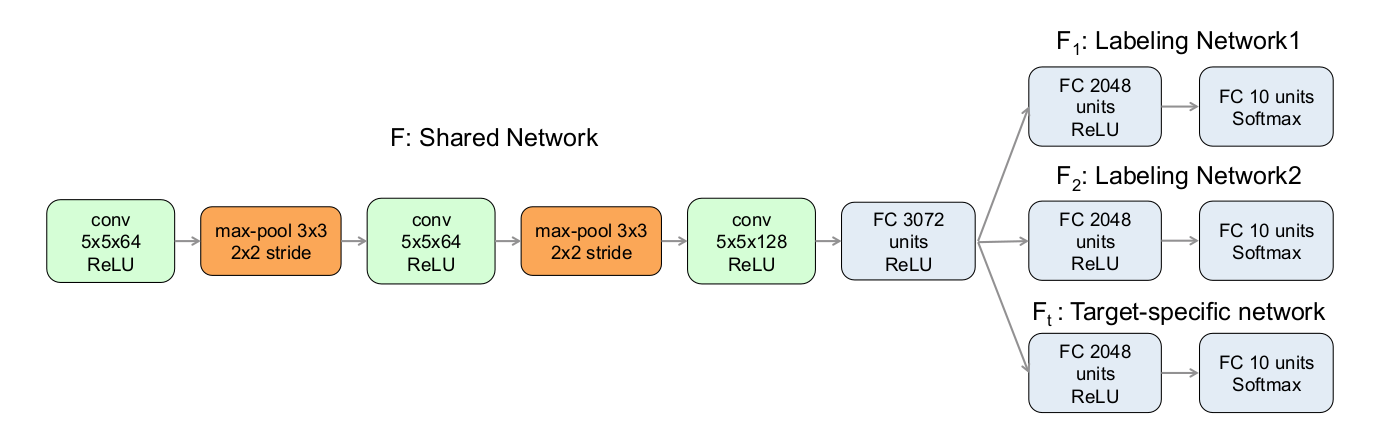
\includegraphics[width=0.8\textwidth]{ATT/Imp_acc.png}
  \caption{Architecture used for SVHN-MNIST domain adaptation. The feature extractor is a CNN with batch normalization in the last convolutional layer, and the classifiers are fully connected layers with batch normalization and dropout.}
  \label{fig:att_implementation}
\end{figure}



%%%%%%%%%%%%%%%%%%%%%%%%%%%%%%%%%%%%%%%%%%%%%%%%%%%%%%%%%%%%


\end{document}